\section{Versuchsaufbau/-durchführung}
Im folgenden Kapitel sollen die wesentlichen Bauteile des Versuchsaufbau beschrieben
werden. Zusätzlich wird das Justage- und Messverfahren vorgestellt.

\subsection{Versuchsaufbau}
\FloatBarrier
Der verwendete Versuchsaufbau ist in Abbildung \ref{fig:aufbau} dargestellt.
\begin{figure}
\centering
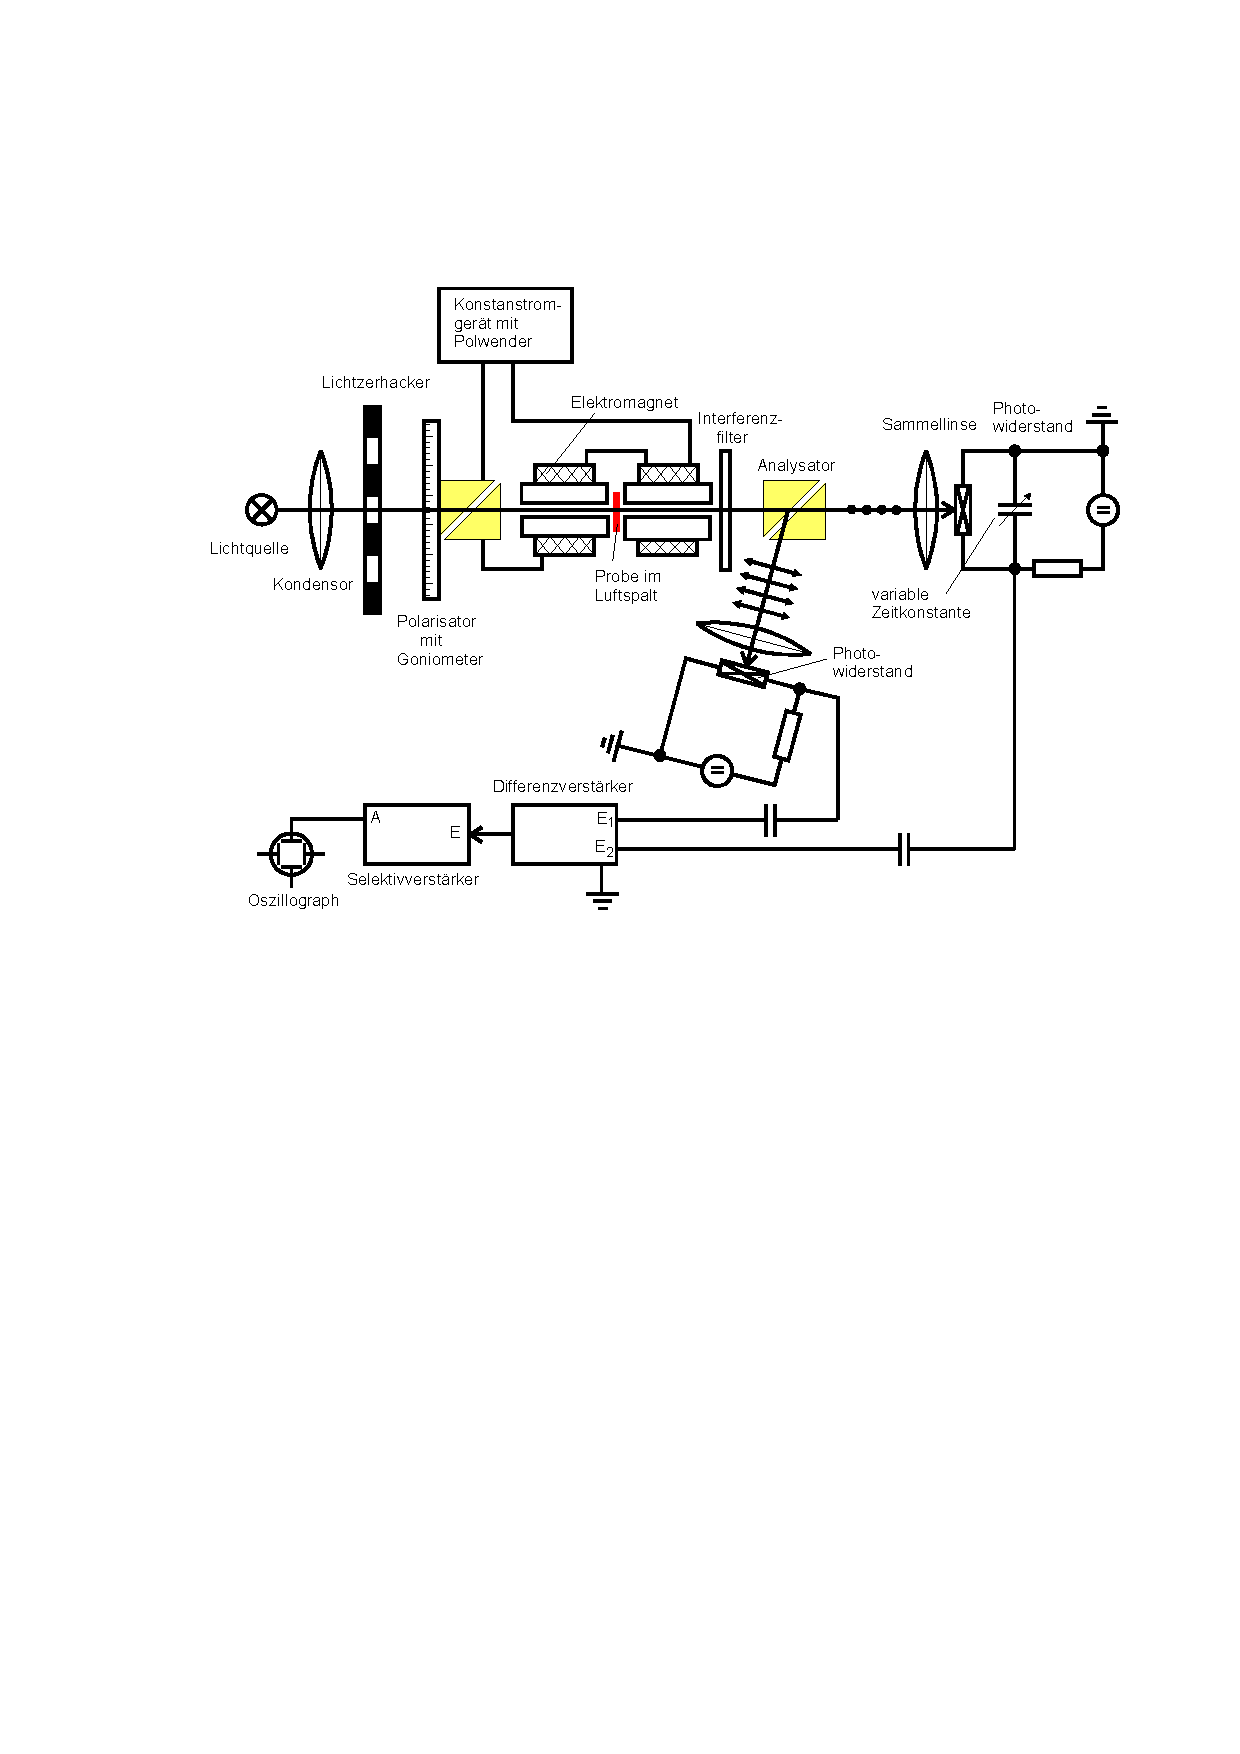
\includegraphics[width=0.7\linewidth]{./content/images/aufbau.pdf}
\caption{Schematische Darstellung des Versuchsaufbaues \cite{anleitungv46}.}
\label{fig:aufbau}
\end{figure}
Das Experiment verwendet als Lichtquelle eine Halogen-Lampe, dessen Emissionsspektrum
hauptsächlich im Infraroten bereich liegt. Das emittierte Licht wird von einer
Kondensorlinse gesammelt und als paralleler Strahl in den weiteren Veruschsaufbau
eingespeißt (vgl. Abbildung \ref{fig:kondensorlinse}).
\begin{figure}
\centering
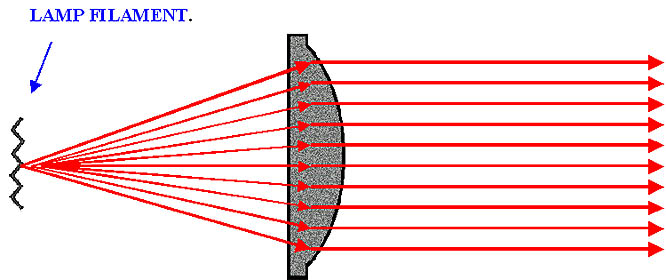
\includegraphics[width=0.45\linewidth]{./content/images/condensor.JPG}
\caption{Schematische Strahlengang von Licht vor und nach einer Kondensorlinse.
Abbildung nach Quelle \cite{kondensorlinse}.}
\label{fig:kondensorlinse}
\end{figure}
Das von der Kondensorlinse gesammelte Licht gelangt über einen Lichtzerhacker in
ein Glan-Thompson-Prisma. Das aus Kalkspat bestehende Prisma erzeugt das
für die Messung notwendige linear polarisierte Licht (vgl. Abb. \ref{fig:glan_thompson_prisma}).
\begin{figure}
\centering
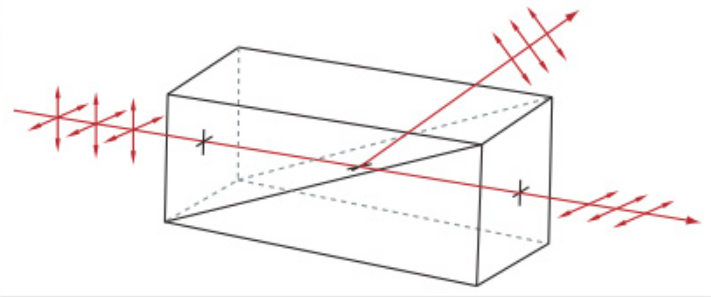
\includegraphics[width=0.5\linewidth]{./content/images/glan_thompson_prisma.png}
\caption{Schematische Darstellung eines Glan-Thompson-Prisma als Strahlenteiler.
Die Polarisationsebenen der beiden austretenden Strahlen stehen orthogonal aufeiannder.
Abbildung nach Quelle \cite{glan_thompson_prisma}.}
\label{fig:glan_thompson_prisma}
\end{figure}
Das polarisierte Licht trifft auf die, sich in einem Magentfeld befindliche,
Probe. Zu betonen ist, dass das Licht parallel zum zeitlich konstanten Magnetfeld
auf die Probe fällt. Als Proben werden zwei n-dotierte
und ein reiner Galliumarsenid Kristalle untersucht. Hierbei unterscheiden sich die
beiden n-dotierten Kristallen in ihrer Dicke und Dotierungstärke. Nach dem Durchqueren
der Probe, wird das Wellenlängenspektrum des Lichts mittels
eins Interferenzfilter auf eine Wellenlänge reduziert. Ein Interferenzfilter
besteht aus zwei semitransparenten Schichten die eine transparentes Dielektrikum
umgeben (vgl. Abb. \ref{fig:interferenzfilter}). Das eintretende Licht wird durch die reflektierenden
Außenschichten mehrmals reflektiert, was zu einer Interferenz führt.
Mit Hilfe dieser Vielzahl-Interferenz ist es möglich, durch Variierung der
Dicke des Filters, nur vereinzelte Wellenlängen passieren zu lassen.
\begin{wrapfigure}{r}{0.5\textwidth}
\centering
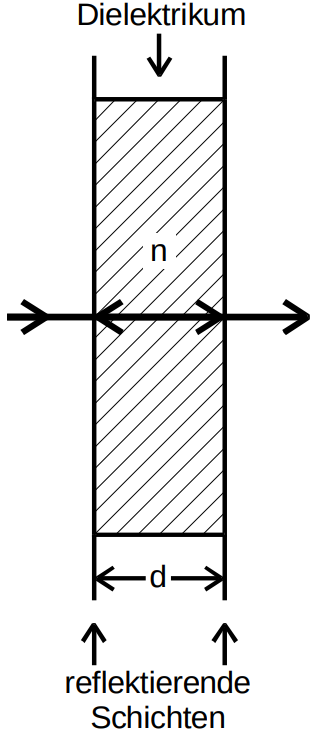
\includegraphics[width=0.35\linewidth]{./content/images/interferenzfilter.png}
\caption{Schmeatischer Aufbau eines Interfernzfilters \cite{anleitungv46}.}
\label{fig:interferenzfilter}
\end{wrapfigure}
Das monochromatische Licht trifft anschließend auf einen zweiten Glan-Thompson-Prisma
der zwei Teilstrahlen unterschiedlicher Polaristation erzeugt. Die Intensität
der beiden ausgehenden Strahlen hängt dabei von der Polarisation des eingehenden
Lichtstrahl ab. Die beiden Teilstrahlen werden mit Hilfe von Sammellinsen auf
jeweils eine Photodiode fokussiert. Die Photodioden transformieren die
Intensität des auftretenden Lichtes in eine Strom. Das Signal der beiden
Photdioden wird auf einen Differenzverstärker gegeben, welcher ,namentgebend,
beide Signale voneinander subtrahiert und die resultierende Differenz verstärkt.
Die dem \emph{Balance Schema} folgende Messmethode bietet eine besonders hohe Genauigkeit.
Das Signal des Differenzverstärkers wird zu einem Selektivverstärker weitergeleitet.
Mit dem Selektivverstärker soll die Genauigkeit der Messung weiter verbessert werden.
Hierzu wird die Verstärkerfrequenz des Selektivverstärkers auf die Frequenz des
Lichtzerhackers eingestellt. Die Abstimmung des Selektivverstärkers auf die
Lichtzerhackerfrequenz verbessert signifikant das Signal-Rauschverhältnis.
Abschließend wird das verstärkte Signal in ein Oszilloskop eingespeißt.

\subsection{Kalibrierung und Messprogramm}
Zu Beginn der Kalirbierung wird überprüft, ob das von den Sammellinsen
fokussierte Licht auf den Sensitivenbereich der jeweiligen Photodioden fällt.
Anschließend wird eine Photodiode mit dem Selektivverstärker verbunden.
Die Verstärkerfrequenz des Selektivverstärkers wird nun solange variiert
bis eine maximale Signalamplitude aud dem Oszilloskop eingestellt wurde.
Nachdem die Verstärkerfrequenz eingstellt wurde, werden beide Photodioden
an den Differenzverstärker angeschlossen.

Die Bestimmung des Polarisationswinkel $\vartheta$ erfolgt mit Hilfe eines
an dem ersten Glan-Thompson-Prisma angebrachten Goniometer. Nachdem einsetzen einer
Probe und eines Filters, wird das Goniometer so lange varriert bis ein Signalminiumun
auf dem Oszilloskop gefunden wird. Der am Gonitmeter eingetsellte Winkel $\vartheta_1$ wird
notiert. Eine Änderung des Magnetfeldes um $2B$ kann durch eine Umpolung des
Magnetfeldes bewirkt werden. Nach der Umpolung wird ein weiteres Mal mit dem
Goniometer ein Minimum gesucht und der dazugehöroge Winkel $\vartheta_2$ notiert.
Aus den beiden vermerkten Winkel ist es nun möglich, den Drehwinkel der Polarisationsebene
$\vartheta$ über den Zusammenhang
\begin{equation}
  \label{eq:theta_aus_messung}
  \vartheta = \frac{1}{2}(\vartheta_1 - \vartheta_2)
\end{equation}
zu bestimmen. Die Winkel $\vartheta_1$ und $\vartheta_2$ werden nun für verschiedene
Interferenzfilter bestimmt. Nach der Vermessung aller Proben ist es möglich die
effektive Massen der Donatorelektron zubestimmen.
Abschließend wird mit Hilfe einer Hallsonde das Magnetfeld im inneren der Spule
vermessen.
\FloatBarrier
